\documentclass[5p,times]{elsarticle}
\usepackage{tikz}
\usepackage{graphicx}
\usepackage{caption}  
\usetikzlibrary{shapes.geometric, arrows.meta, positioning}

\usetikzlibrary{fit, backgrounds}
\usepackage{amsmath}


\tikzstyle{block} = [rectangle, draw=black, fill=blue!10, minimum width=4cm, minimum height=0.9cm, font=\small, text centered]
\tikzstyle{branch} = [rectangle, draw=black, fill=gray!10, minimum width=3.8cm, minimum height=0.9cm, font=\small, text centered]
\tikzstyle{local} = [rectangle, draw=black, fill=orange!15, minimum width=4cm, minimum height=0.9cm, font=\small, text centered]
\tikzstyle{global} = [rectangle, draw=black, fill=purple!10, minimum width=4cm, minimum height=0.9cm, font=\small, text centered]
\tikzstyle{arrow} = [thick, ->, >=stealth]


\begin{document}



\begin{figure*}[ht]
\centering
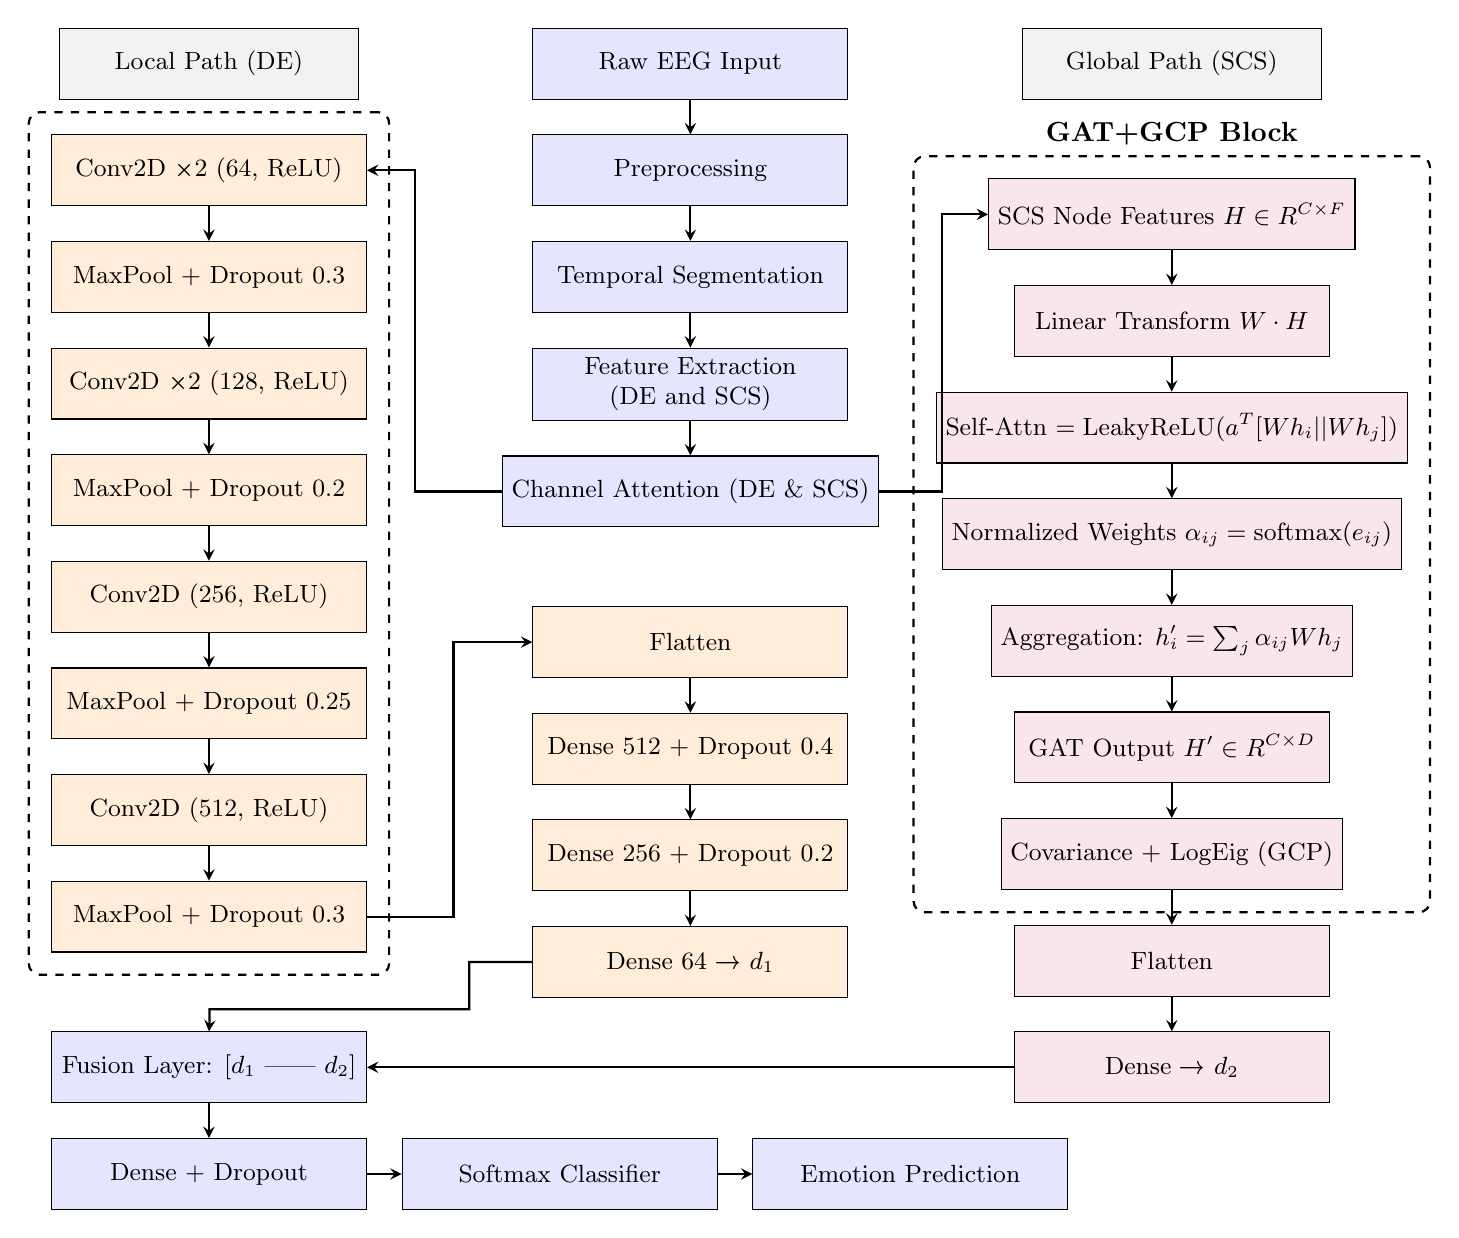
\begin{tikzpicture}[node distance=0.44cm]

% Input flow
\node (input) [block] {Raw EEG Input};
\node (prep) [block, below=of input] {Preprocessing};
\node (segment) [block, below=of prep] {Temporal Segmentation};
\node (features) [block, below=of segment, align=center] {Feature Extraction\\ (DE and SCS)};
\node (attention) [block, below=of features] {Channel Attention (DE \& SCS)};

% Local branch
\node (local_label) [branch, left=2.2 cm of input] {Local Path (DE)};
%\node (cnn) [local, below=of local_label] {2D CNN Layers};
%\node (flatten1) [local, below=of cnn] {Flatten + Dense → $d_1$};
% Local CNN Blocks (DE)
\node (conv1) [local, below=of local_label] {Conv2D ×2 (64, ReLU)};
\node (pool1) [local, below=of conv1] {MaxPool + Dropout 0.3};

\node (conv2) [local, below=of pool1] {Conv2D ×2 (128, ReLU)};
\node (pool2) [local, below=of conv2] {MaxPool + Dropout 0.2};

\node (conv3) [local, below=of pool2] {Conv2D (256, ReLU)};
\node (pool3) [local, below=of conv3] {MaxPool + Dropout 0.25};

\node (conv4) [local, below=of pool3] {Conv2D (512, ReLU)};
\node (pool4) [local, below=of conv4] {MaxPool + Dropout 0.3};

\node (flatten) [local, below= 1 cm of attention] {Flatten};
\node (dense1) [local, below=of flatten] {Dense 512 + Dropout 0.4};
\node (dense2) [local, below=of dense1] {Dense 256 + Dropout 0.2};
\node (dense3) [local, below=of dense2] {Dense 64 → $d_1$};

\node [draw=black, thick, dashed, inner sep=8pt, fit=(conv1)(pool4), label=above:{\textbf{}}, fill=none, rounded corners] {};



% Global branch
\node (global_label) [branch, right=2.2cm of input] {Global Path (SCS)};
\node (gat_in) [global, below=1 cm of global_label] { SCS Node Features $H \in \mathbb{R}^{C \times F}$};
\node (gat_linear) [global, below=of gat_in] {Linear Transform $W \cdot H$};
\node (gat_attn) [global, below=of gat_linear] {Self-Attn $= \text{LeakyReLU}(a^T [W h_i || W h_j])$};
\node (gat_softmax) [global, below=of gat_attn] {Normalized Weights $\alpha_{ij} = \text{softmax}(e_{ij})$};
\node (gat_agg) [global, below=of gat_softmax] {Aggregation: $h'_i = \sum_j \alpha_{ij} W h_j$};
\node (gat_out) [global, below=of gat_agg] {GAT Output $H' \in \mathbb{R}^{C \times D}$};

%\node (gat) [global, below=of gat_out] {Graph Attention (GAT)};
\node (gcp) [global, below=of gat_out] {Covariance + LogEig (GCP)};
\node (flattenn) [global, below=of gcp]  {Flatten};
\node (flatten2) [global, below=of flattenn] {Dense → $d_2$};
\node [draw=black, thick, dashed, inner sep=8pt, fit=(gat_in)(gat_attn)(gat_out)(gcp), label=above:{\textbf{GAT+GCP Block}}, fill=none, rounded corners] {};

% Fusion and output
\node (fusion) [block, below= 1 cm of pool4] {Fusion Layer: [$d_1$ || $d_2$]};
\node (densecls) [block, below= of fusion] {Dense + Dropout};
\node (softmax) [block, right=of densecls] {Softmax Classifier};
\node (output) [block, right=of softmax] {Emotion Prediction};

% Flow arrows
\draw [arrow] (input) -- (prep);
\draw [arrow] (prep) -- (segment);
\draw [arrow] (segment) -- (features);
\draw [arrow] (features) -- (attention);

% Local path arrows
%\draw [arrow] (attention.west) -- ++(-1.5,0) |- (cnn);
%\draw [arrow] (cnn) -- (flatten1);
%\draw [arrow] (flatten1) -| (fusion);
\draw [arrow] (attention.west) -- ++(-1.1,0) |- (conv1);
\draw [arrow] (conv1) -- (pool1);
\draw [arrow] (pool1) -- (conv2);
\draw [arrow] (conv2) -- (pool2);
\draw [arrow] (pool2) -- (conv3);
\draw [arrow] (conv3) -- (pool3);
\draw [arrow] (pool3) -- (conv4);
\draw [arrow] (conv4) -- (pool4);
\draw [arrow] (pool4.east) - ++(1.1,0) |- (flatten.west);
\draw [arrow] (flatten) -- (dense1);
\draw [arrow] (dense1) -- (dense2);
\draw [arrow] (dense2) -- (dense3);
%\draw [arrow] (dense3.west) -- (1.1,0) ++|-  (fusion);
\draw [arrow] (dense3.west) -- ++(-0.8,0) -- ++(0,-0.6) -- ++(-3.3,0) -- ++(0,-0.2) -- (fusion.north);

\draw [arrow] (attention.east) -- ++(0.8,0) |- (gat_in);
\draw [arrow] (gat_in) -- (gat_linear);
\draw [arrow] (gat_linear) -- (gat_attn);
\draw [arrow] (gat_attn) -- (gat_softmax);
\draw [arrow] (gat_softmax) -- (gat_agg);
\draw [arrow] (gat_agg) -- (gat_out);
% Global path arrows

\draw [arrow] (gat_out) -- (gcp);
\draw [arrow] (gcp) -- (flattenn);
\draw[arrow] (flattenn) -- (flatten2);
\draw [arrow] (flatten2.west) -- ++(-1.5,0) |-  (fusion.east);




% Output arrows
\draw [arrow] (fusion) -- (densecls);
\draw [arrow] (densecls.east) -- (softmax.west);
\draw [arrow] (softmax.east) -- (output.west);

\end{tikzpicture}
\caption{DAFNet architecture: a dual-path network combining a local 2D CNN path using DE features and a global path using GAT and GCP over SCS features. Outputs from both paths are fused for final emotion classification.}
\label{fig:block_diagram}
\end{figure*}
\end{document}